\documentclass[11pt, oneside]{article}   	% use "amsart" instead of "article" for AMSLaTeX format

% \usepackage{draftwatermark}
% \SetWatermarkText{Draft}
% \SetWatermarkScale{6}
% \SetWatermarkLightness {0.90} 
%\SetWatermarkColor[rgb]{0.7,0,0}


\usepackage{geometry}                		% See geometry.pdf to learn the layout options. There are lots.
\geometry{letterpaper}                   		% ... or a4paper or a5paper or ... 
%\geometry{landscape}                		% Activate for for rotated page geometry
%\usepackage[parfill]{parskip}    		% Activate to begin paragraphs with an empty line rather than an indent
\usepackage{graphicx}				% Use pdf, png, jpg, or eps� with pdflatex; use eps in DVI mode
								% TeX will automatically convert eps --> pdf in pdflatex		
\usepackage{amssymb}
\usepackage{mathrsfs}
\usepackage{hyperref}
\usepackage{url}
\usepackage{subcaption}
\usepackage{authblk}
\usepackage{amsmath}
\usepackage{mathtools}
\usepackage{graphicx}
\usepackage[export]{adjustbox}
\usepackage{fixltx2e}
\usepackage{hyperref}
\usepackage{alltt}
\usepackage{color}
\usepackage[utf8]{inputenc}
\usepackage[english]{babel}
\usepackage{float}

 
\newtheorem{theorem}{Theorem}[section]
\newtheorem{corollary}{Corollary}[theorem]
\newtheorem{lemma}[theorem]{Lemma}

\newcommand{\argmax}{\operatornamewithlimits{argmax}}
\newcommand{\argmin}{\operatornamewithlimits{argmin}}


\title{Comments on "Networkless: Current Status \\ and Future Approaches"\footnote{This report is a deliverable for Project Number HE2017070001.}}
\author{David Meyer \\
dmm@1-4-5.net}

\date{Last update: \today}							% Activate to display a given date or no date


\begin{document}
\maketitle

\section{Introduction} 
\label{sec:intro}
The document provides a review of the "Networkless: Current Status and Future Approaches" deck that was discussed on 09/19/2018. The deck is organized into four sections:
\begin{itemize}
\item Background: Human cost issue
\item IETF Standardization Work (ANIMA)
\item Ongoing Research Projects
\item Roadmap
\end{itemize}

\bigskip
\noindent
The approach taken in this document (and in the "tableless" document) will be to review each slide and provide comments where useful. 
These comments will be organized into three categories: 

\begin{itemize}
\item Feedback the technical aspects of each slide. I will include the slide where doing so would provide additional information
\item Feedback  on where we might find colleagues (industry, academia, or other)
\item Marketing strategies
\end{itemize}

\bigskip
\noindent
The approach taken here is to review each slide in light of these three categories. I will take the deck slide by slide, providing comments where appropriate. Here page number is equivalent 
to slide number. I will also include a section on Nits (editorial and non-technical comments) where appropriate.

\bigskip
\noindent
Finally Section \ref{sec:conclusions} provides a few conclusions.

\section{Slide 4}
\label{sec:slide4}

Slide 4 introduces the long studied problem of growing network complexity and the associated growth in configuration information. As mentioned in the slide, this problem is being
addressed in part by the "Autonomic Networking" (AN) activity in the IETF. There are many research projects in this space (see e.g., \url{https://en.wikipedia.org/wiki/Autonomic_networking}
for a reasonably up to date list).

\begin{figure}
\center{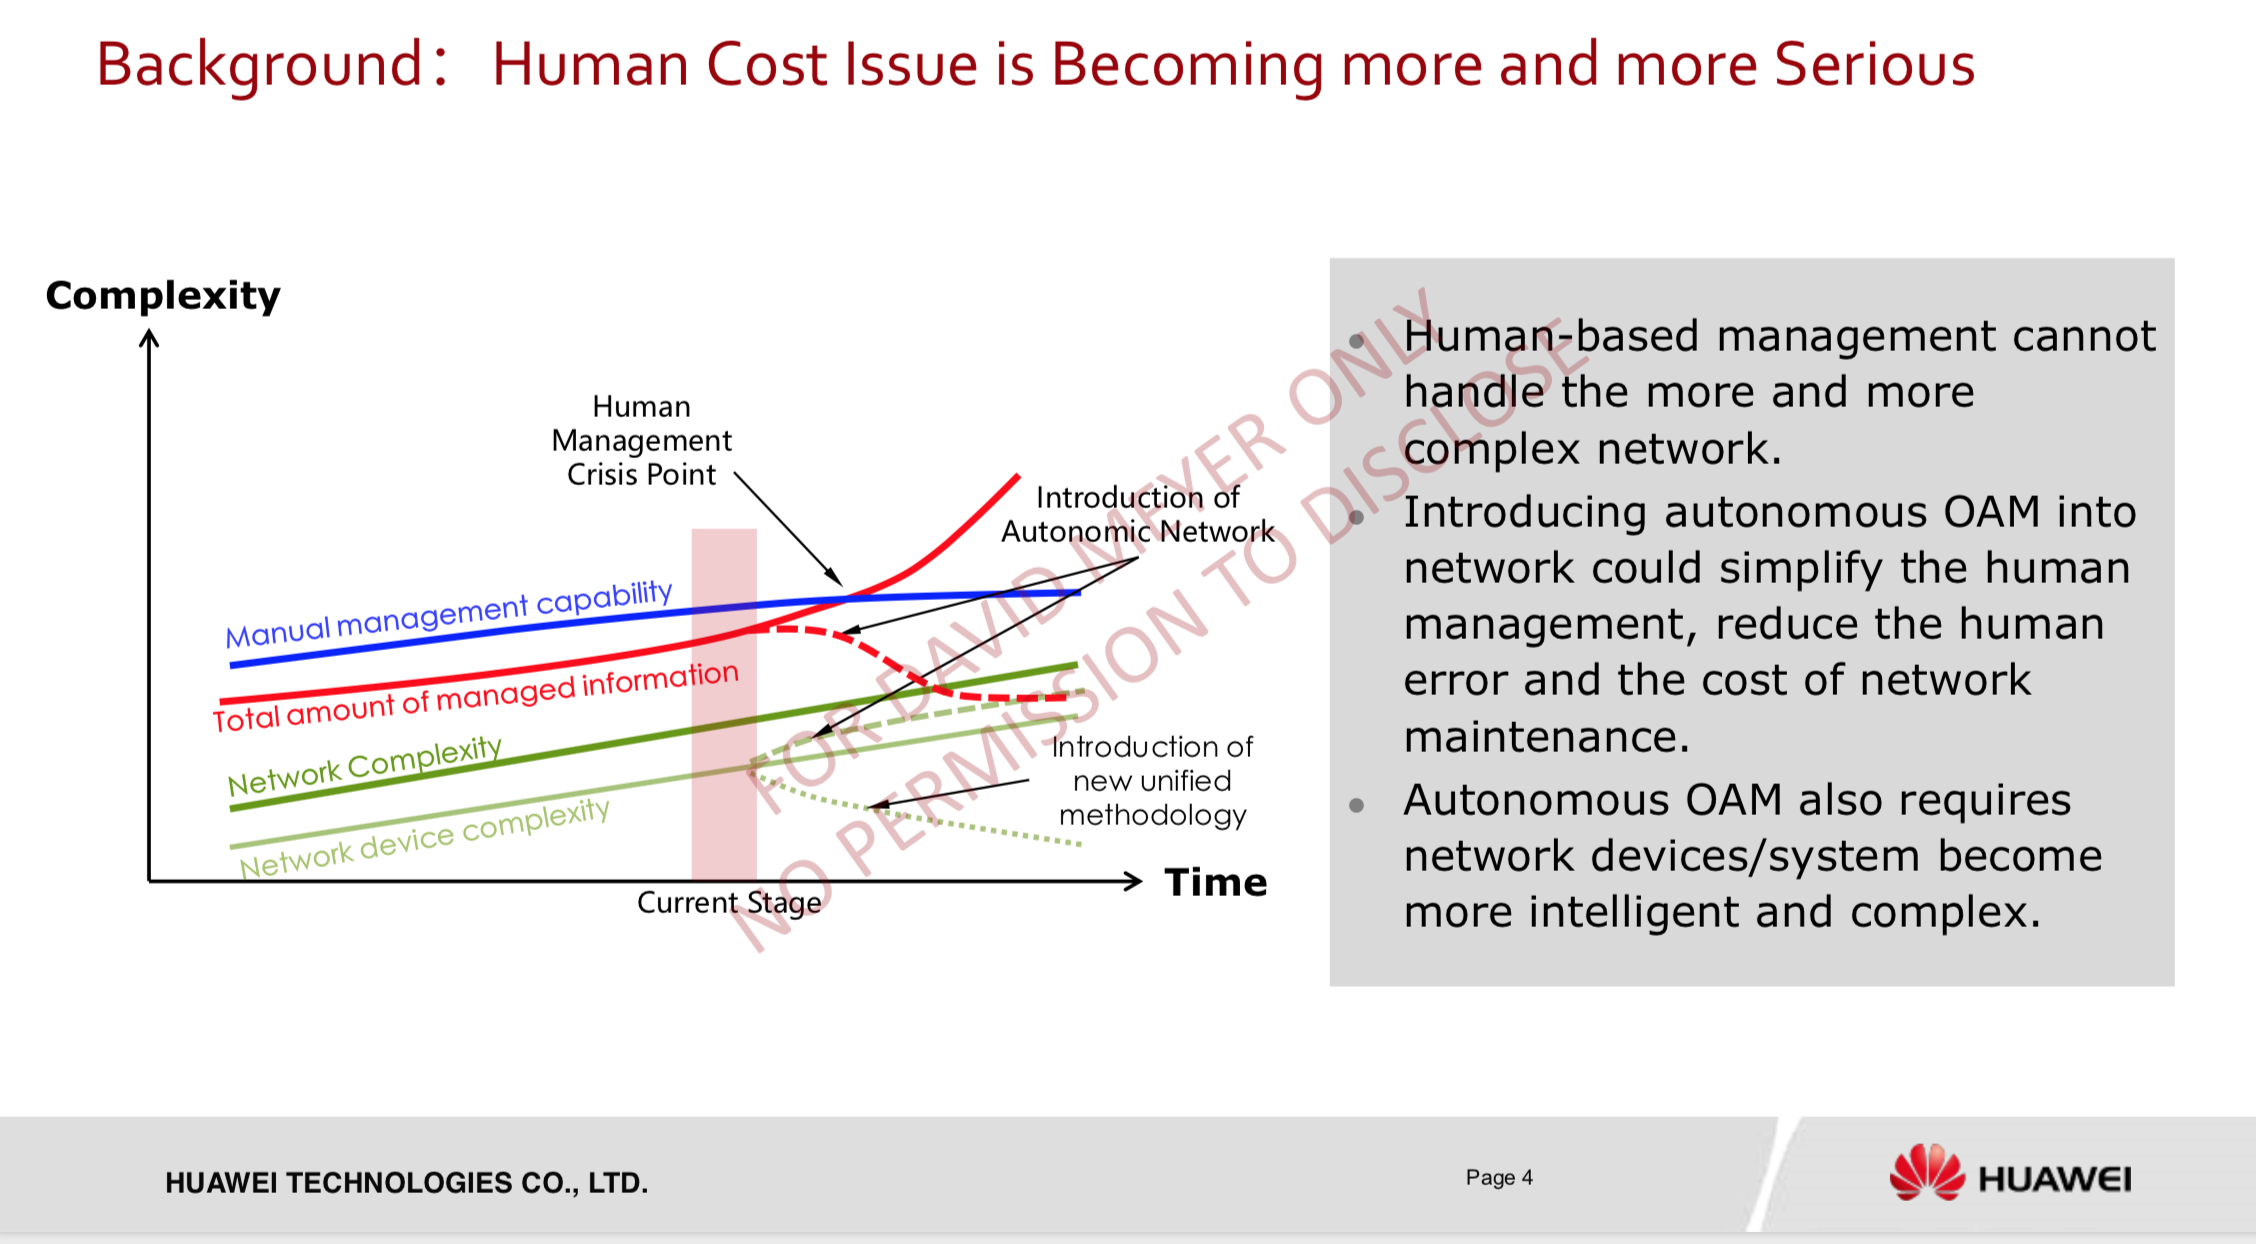
\includegraphics[scale=0.35, frame] {images/slide4.png}}
\caption{Slide 4}
\label{fig:slide4}
\end{figure}


\subsection{Technical Feedback}
\label{slide4:technical_feedback}
The "Current Stage" on the time axis is confusing. I presume you mean  "Present Time" or similar. In addition,  the pink block representing "Current Stage" is confusing. Be more 
precise in what is meant. In addition, it looks like "Introduction of Autonomic Networking" is in the future, while many have already rolled out some AN capability. See e.g. 
\url{https://www.cisco.com/c/en/us/td/docs/switches/metro/me3600x_3800x/software/release/15-4_2_S/configuration/guide/3800x3600xscg/autonomic_net.html}. In addition,
"Introduction of new unified methodology" is also vague. What is it, why is it unified, and why are the relative time scales as depicted. In general, I would add citations supporting
the timelines shown.

\subsection{Possible Collaborators}
\label{slide4:possible_collaborators}
In the AN space, the IETF is a reasonable place to look for collaborators. 

\subsection{Marketing Strategies}
\label{slide4:marketing_strategies}
This of course depends on what Huawei products and services have AN capability. That said, this kind of high-level, marketing approach is ideal for conferences like the ONS,
Layer123, and the Upperside conferences. These are largely marketing events and as such should be attended "C-level" Huawei representatives and field marketing people.

\subsection{Nits}
\label{slide4:nits}
N/A

\section{Slide 5}
\label{sec:slide5}

Slide 5 introduces what looks like a "functionality timeline". The first parts of the timeline are covered by AN; the "Upgrade" parts are still research.


\subsection{Technical Feedback}
\label{slide5:technical_feedback}
First, "Upgrade" seems to be the wrong term. What we are really talking about is changing the way we do networking, so I would perhaps change that to "Future". This 
would also address a problem with time not being explicitly represented.

\subsection{Possible Collaborators}
\label{slide5:possible_collaborators}
Again, for "Self-Organization" and "Self-Configuration"  we would expect this to be handled by AN, making the IETF the right place for this. On the other hand, the other 
categories require new approaches, possibly involving Machine Learning (ML)  \cite{2017arXiv170908339W}. Hence there is wide scope for collaboration. As we have observed
the uptake of ML in networking has been slow; there are several reasons for this, including missing skill sets, data sets, and the difficult problem of dynamic networks. 
Innovative collaborators would be physicists, control theorists, and biologists. I have spoken about this problem on many occasions (see for example 
\url{http://www.1-4-5.net/~dmm/talks/2015/hoti.pptx}).

\subsection{Marketing Strategies}
\label{slide5:marketing_strategies}
This again depends on what work Huawei has actually done. The situation where Huawei has products with AN capability is handled Section \ref{slide4:marketing_strategies}.
Huawei should also try to establish leadership in the ML space by publishing results, at least on \url{https://arxiv.org}. Better would be publication in peer-reviewed publications.
In addition, making code and data sets available under some open-source license. Technical talks demonstrating of ML techniques on network-oriented use cases would also
be helpful.
    
\subsection{Nits}
\label{slide5:nits}
"balance the traffic in different links in the network" should be "balance the traffic \emph{on} different links".


\section{Slides 7-13}
\label{sec:slide7-13}

Slides 7-13 review the standard ANIMA scenario. I'll just point out here that the typical IETF ideal of using "re-useable components", while being
completely reasonable in the near term,  may not be the right long term approach\footnote{For example, while "intent" is an important current
technology direction, the longer term direction is likely to be less human-mediated.}.


\subsection{Technical Feedback}
\label{slide7:technical_feedback}
N/A

\subsection{Possible Collaborators}
\label{slide7:possible_collaborators}
N/A

\subsection{Marketing Strategies}
\label{slide7:marketing_strategies}
N/A

\subsection{Nits}
\label{slide7:nits}

There appears to be extra space after "indicates that Anima is not a "Clean Slate"" and 
before the comma in "Anima aims at developing some "re-useable components"" on slide 7. In addition, "Anima" is 
actually an acronym and as such should be capitalized (ANIMA). 

\section{Slide 14}
\label{sec:slide14}

Slide 14 updates slide 5 by adding ASA components for both Self-Organization and Self-Configuration. The comment "In theory, Anima ASA can almost cover every aspect of "Self-"
has a few issues. First, it seems it should say "Self-*". Second, "in theory..." -- what theory, and how exactly can ANIMA ASA cover every aspect of Self-*. Finally,  Self-* is not
defined.

\subsection{Technical Feedback}
\label{slide7:technical_feedback}
N/A

\subsection{Possible Collaborators}
\label{slide7:possible_collaborators}
N/A

\subsection{Marketing Strategies}
\label{slide7:marketing_strategies}
N/A

\subsection{Nits}
\label{slide7:nits}

N/A

\section{Slide 17}
\label{sec:slide17}

Main comment here is that if it is important to say that domains (RSG, ASG, CSG) can be discriminated by some form of clustering, it would be nice to see 
how it actually works. The slide doesn't give that information. 

\subsection{Technical Feedback}
\label{slide17:technical_feedback}
Using clustering is a good idea if it works since (a). it an unsupervised approach, and (b). it is very simple. However, the slide does not tell the reader why
this works (XMEANS) or how. In addition, the statement "RSG/ASG/CSG domains are highly relevant to routing domains and service configuration policies" seems 
obvious, and doesn't really add anything. Again, better (more) explanation of why and how this works would be helpful.

\subsection{Possible Collaborators}
\label{slide17:possible_collaborators}
N/A

\subsection{Marketing Strategies}
\label{slide17:marketing_strategies}
N/A

\subsection{Nits}
\label{slide17:nits}
N/A

\begin{figure}
\center{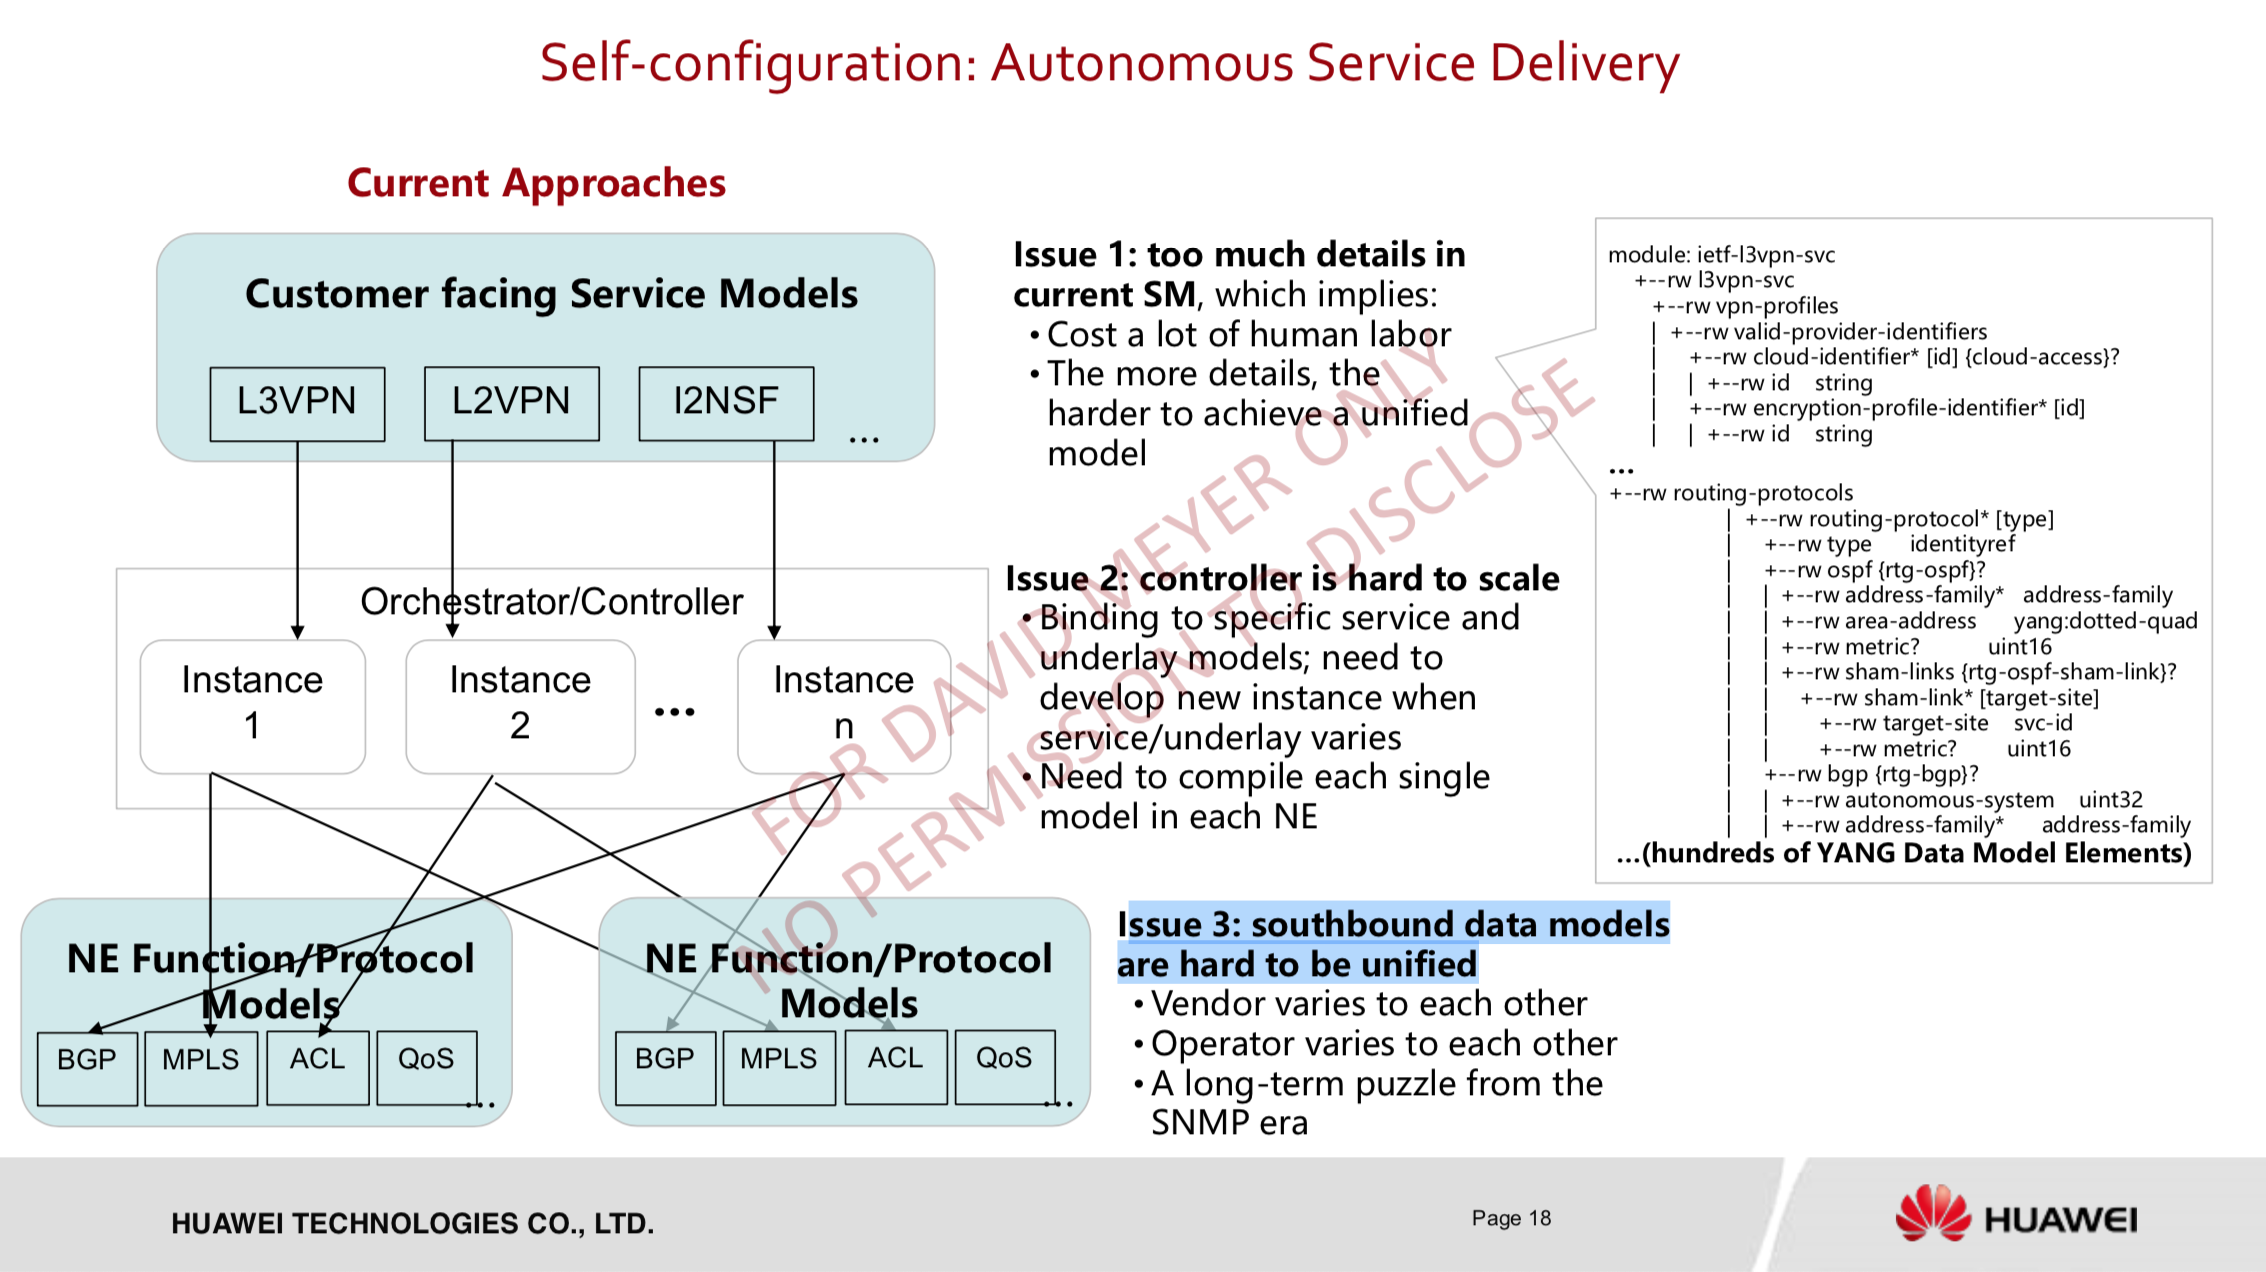
\includegraphics[scale=0.35, frame] {images/slide18.png}}
\caption{Slide 18}
\label{fig:slide18}
\end{figure}


\section{Slide 18}
\label{sec:slide18}

Slide 18 is a nice slide. 

\subsection{Technical Feedback}
\label{slide18:technical_feedback}
N/A

\subsection{Possible Collaborators}
\label{slide18:possible_collaborators}
N/A

\subsection{Marketing Strategies}
\label{slide18:marketing_strategies}
N/A

\subsection{Nits}
\label{slide18:nits}
\begin{itemize}
\item Issue 1: too much details in current SM, which implies:
\begin{itemize}
\item Cost a lot of human labor
\item The more details, the harder to achieve a unified model
\end{itemize}
What we're trying to say is that, in addition to the manual aspects of the current SM, the model is too detailed. This is a computational complexity argument that 
should be made explicit. How to solve this? One way, as pointed out here, is to add hierarchy. The same can be said of Reinforcement Learning
\cite{2018arXiv181001257N,}.   Adding a bit about the need for abstraction to make the problem computable would be helpful.
\item Issue 3: southbound data models are hard to be unified \\ Might say "Issue 3:  unifying southbound data models is difficult".
\end{itemize}

Slide 19 appears to address many of my issues with slide 18.

\begin{figure}
\center{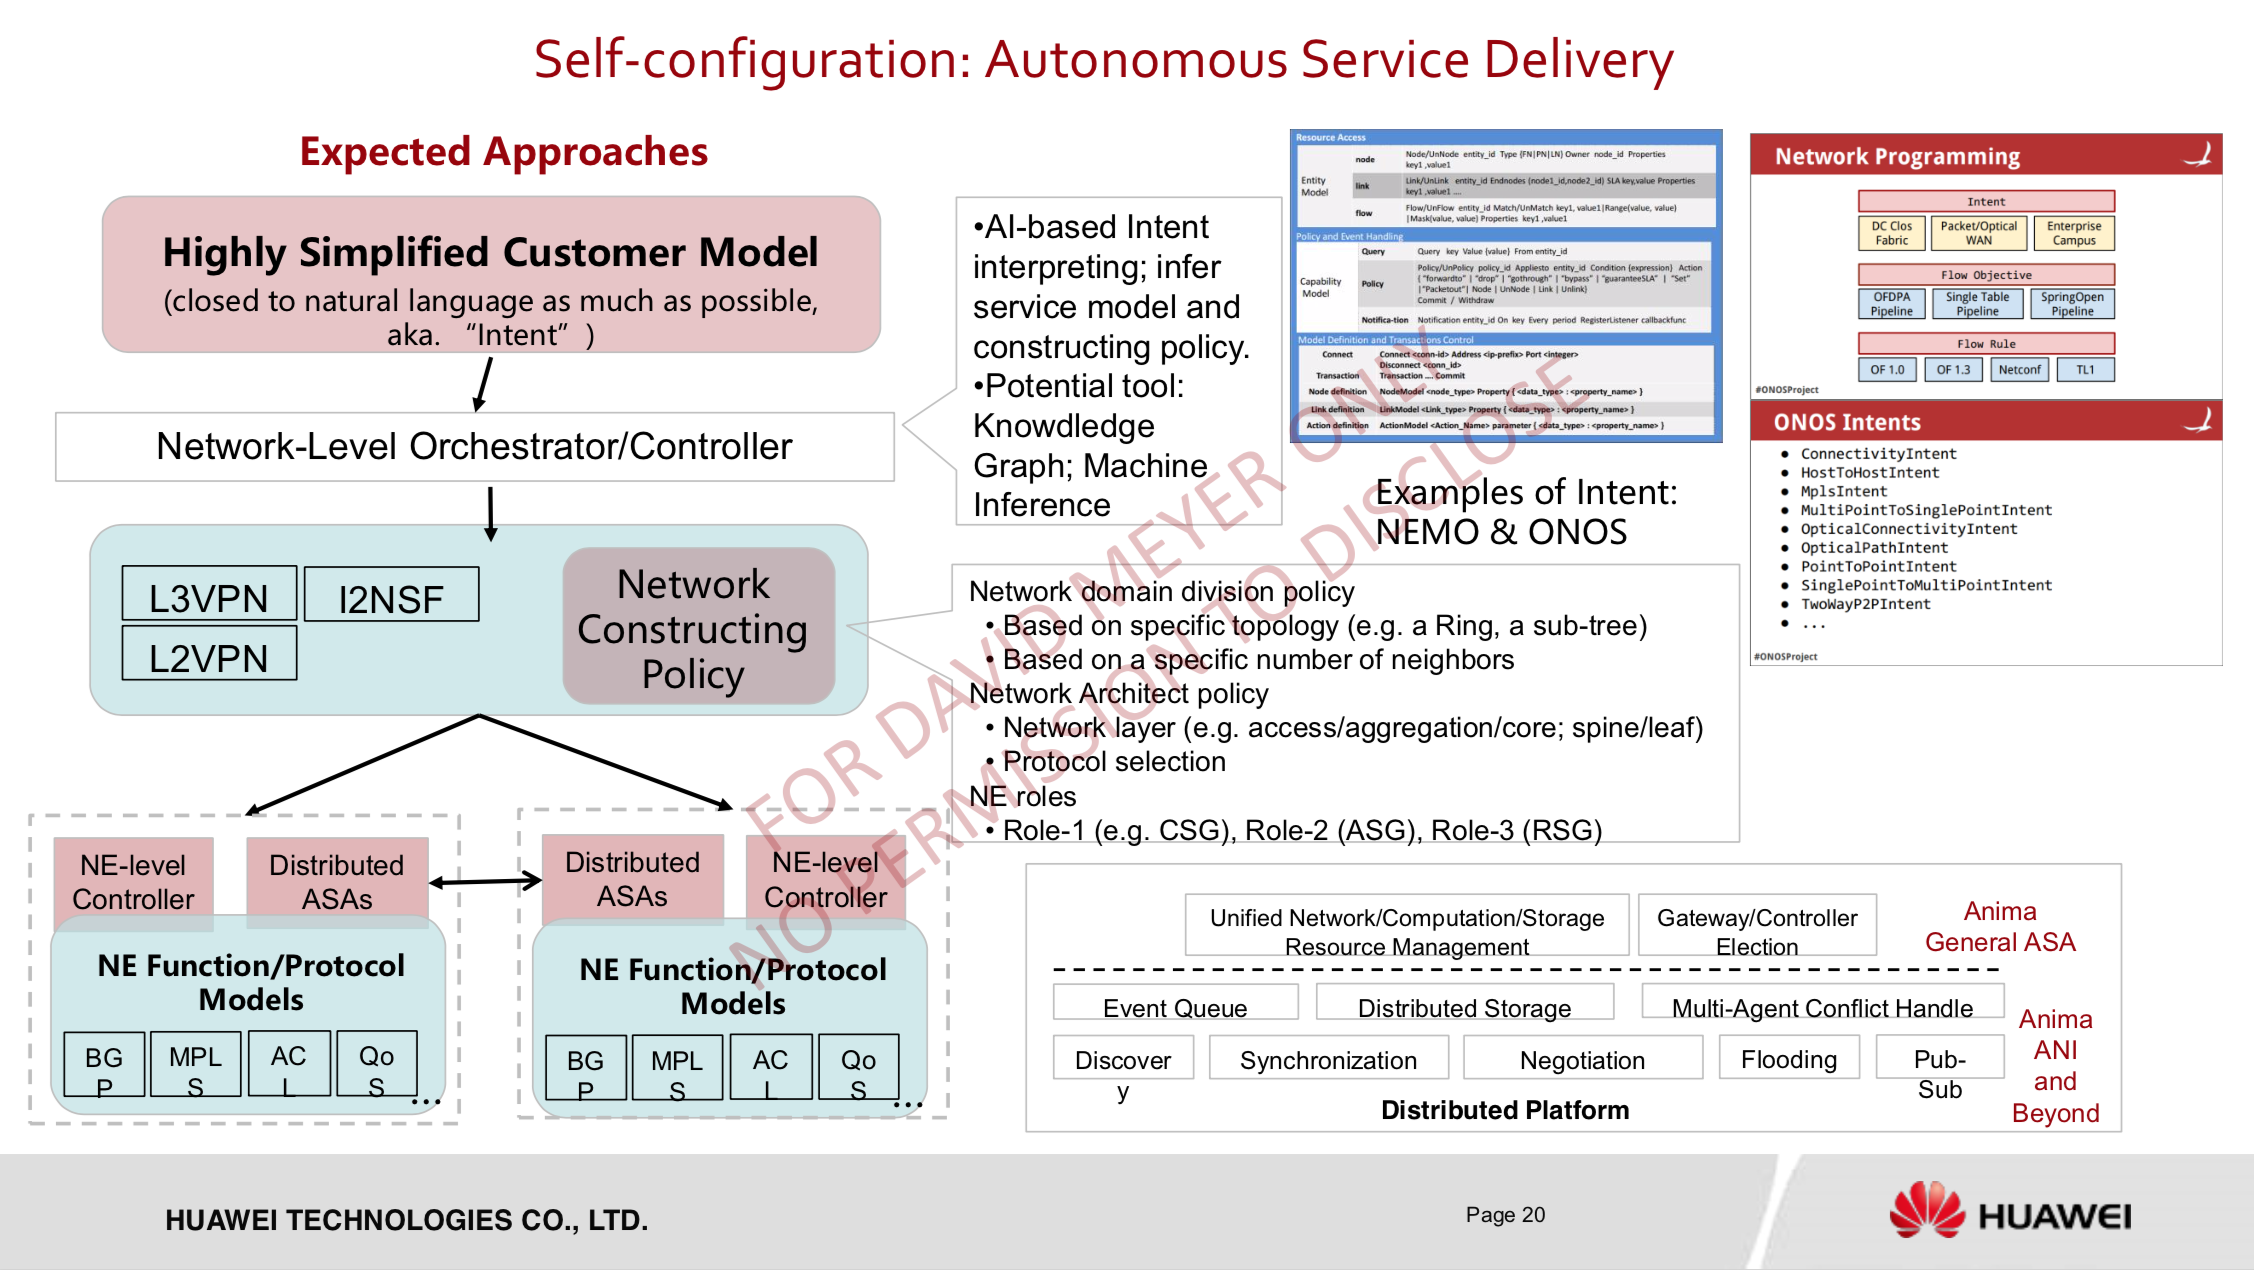
\includegraphics[scale=0.35, frame] {images/slide20.png}}
\caption{Slide 20}
\label{fig:slide20}
\end{figure}


\section{Slide 20}
\label{sec:slide20}

Just an aesthetic comment: the slide is very busy. Perhaps break it into two slides.

\subsection{Technical Feedback}
\label{slide20:technical_feedback}
The comments "AI-based Intent interpreting; infer service model and constructing policy. Potential tool: Knowdledge Graph; Machine Inference" have a few issues.
First (nit): Knowdledge is misspelled. Second, what is "AI-based Intent interpreting", and how does it work? What data is needed? How much compute is required?
Can it be updated efficiently? And how can a Knowledge Graph be used?

\subsection{Possible Collaborators}
\label{slide20:possible_collaborators}
Everyone is networking wants to crack these problems in the ML space. Have you considered working with RedHat?

\subsection{Marketing Strategies}
\label{slide20:marketing_strategies}
In general, I would not suggest marking strategies if there are no products demonstrating the technology approach. However, given
the hype around ML it would be useful to get ML solutions that are close to product in front of customers at an event like the ONS. A combination of
marketing of this type with academic papers which demonstrate advancements in the field would be very good.

\subsection{Nits}
\label{slide20:nits}
See Section \ref{slide20:technical_feedback}.


\section{Slide 21}
\label{sec:slide21}

General comments: The slide is busy. In general more pictures and less works are better. 

\subsection{Technical Feedback}
\label{slide21:technical_feedback}
A couple of things. The PTC and PEFT algorithms are not defined. In addition, "Use AI algorithm for traffic prediction": what AI algorithm, what data is required, how much
compute, can it be dynamically updated, ...In addition, how dynamic can these algorithms be made \cite{Walraven:2016:TFO:2937770.2937891}?  For example, can they 
respond to sub-millisecond changes in congestion (micro-bursts) or topology? Slide 22 gives a nice description of one of the problems to be solved here.

\subsection{Possible Collaborators}
\label{slide21:possible_collaborators}
N/A

\subsection{Marketing Strategies}
\label{slide21:marketing_strategies}
N/A

\subsection{Nits}
\label{slide21:nits}
N/A


\section{Slide 23}
\label{sec:slide23}

Again, the slide is busy. Also lots of acronyms that aren't defined/expanded (e.g. FCT). 

\subsection{Technical Feedback}
\label{slide23:technical_feedback}

Reinforcement Learning (RL) is an obvious approach here. I'll just mention here that "Neural Network based reinforcement learning" is a bit confusing, since there
really isn't any other way to do the RL here; table based approached won't scale \cite{Melo:2008:ARL:1390156.1390240,}. I would just say Deep Reinforcement 
Learning (which is taken to mean RL with function approximation via neural networks for both the policy and value networks). Again, questions like what simulator is 
used (since its RL) and how much data do you need, especially if the data are high-dimension. In addition, it would be interesting/important to know what kind of 
variance the estimators have, and if the variance is too high, how to reduce it (e.g. via  control variates \cite{Andradottir:1993:VRT:174153.174154, 2016arXiv161101142G}).


\subsection{Possible Collaborators}
\label{slide23:possible_collaborators}
N/A

\subsection{Marketing Strategies}
\label{slide23:marketing_strategies}
N/A

\subsection{Nits}
\label{slide23:nits}
N/A

\begin{figure}
\center{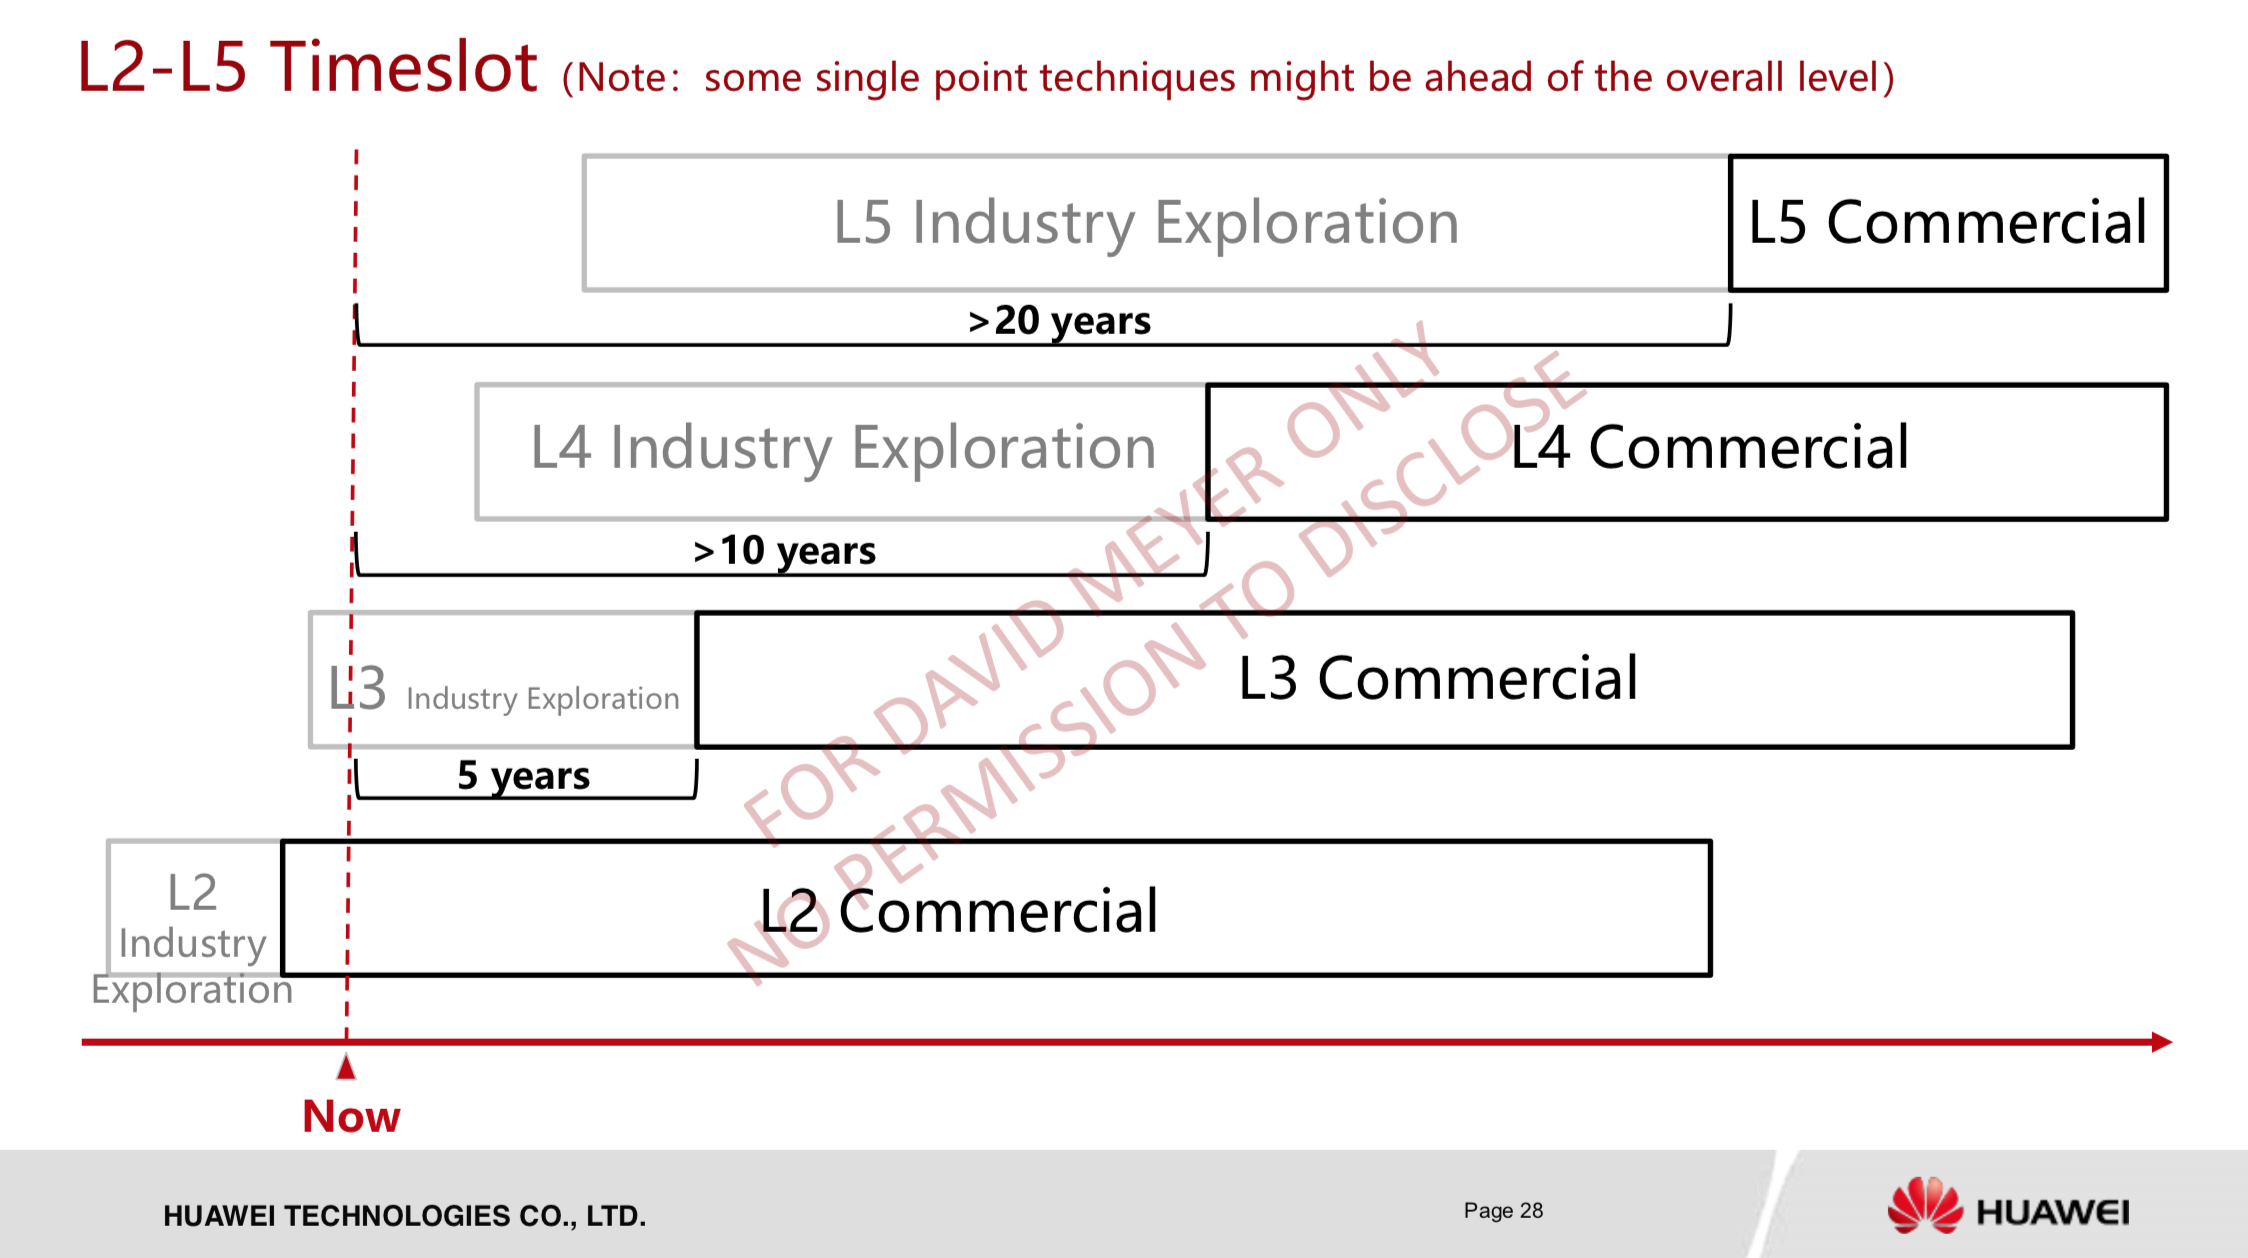
\includegraphics[scale=0.35, frame] {images/slide28.png}}
\caption{Slide 28}
\label{fig:slide28}
\end{figure}



\section{Slide 27}
\label{sec:slide27}

I like slide 27. I would move it forward in the deck. One approach:  Early in the deck briefly describe what autonomic networking is and introduce the self-* terminology 
and then use slide 27. This would be useful closer to the front of the deck. Same with slide 28\footnote{Note that slide 28 uses a vertical line labelled "Now", 
as opposed to "Current Stage" in slide 4.}.


\subsection{Technical Feedback}
\label{slide27:technical_feedback}
How were the time frames selected? 20 years in the future seems quite distant.

\subsection{Possible Collaborators}
\label{slide27:possible_collaborators}
N/A

\subsection{Marketing Strategies}
\label{slide27:marketing_strategies}
N/A

\subsection{Nits}
\label{slide27:nits}
N/A

\section{Conclusions}
\label{sec:conclusions}
The ideas behind "networkless" cleanly fit into the ANIMA framework. This is good, giving access to collaboration and leadership in the IETF and beyond. However, my
basic concern is that ANIMA (and the IETF in general) is relatively conservative (e.g. "re-useable components"). This again is good in the short term;
however, my view of the intermediate term future is different. For example, while "intent based networking" is the current approach, if ML becomes useful in networking (this
hasn't been proven out yet), I expect ML "agents" to develop their own languages; an example would be the so-called "interlinuga" we find in Google Translate. See 
\url{https://ai.googleblog.com/2016/11/zero-shot-translation-with-googles.html}. What we need is a solid theory of network (just as we have a theory of how vision
works (Convolutional Neural Networks) or how languages are processed) combined with efficient unsupervised learning techniques\footnote{It seems unlikely that the network 
space will develop supervised learning datasets like ImageNet \cite{imagenet_cvpr09}.} that allow for transfer learning\footnote{If we can't do transfer
learning then every network is a one-off, and of course we don't want that.}.


\bigskip
\noindent
Regarding marketing and promotion, this should be based on solid results and products. The ideas here are very good, and could be described at a conference like ONS, Layer123, etc.
or at the IETF.  However, what I've seen here is not sufficiently detailed to be presented, for example, at a academic ML conference. More publications (even if on arXiv), demos, 
source code and data would go a long way towards making marketing and promotion more effective. A deeper dive on the technical aspects of this work and its maturity inside Huawei
would help refine my thinking here.


\newpage
\bibliographystyle{ieeetr}
\bibliography{/Users/dmm/papers/huawei/bib/huawei.bib}



\end{document} 
